\chapter{Los registros existentes}\label{sec:chapterVI}
\addcontentsline{toc}{chapter}{Los registros existentes}

En el laboratorio remoto se ha registrado la actividad de $7$ años consecutivos (desde el curso académico $1516$ al $2122$). Un ejemplo de las interacciones almacenadas puede verse en la Tabla \ref{tab:example}.

\begin{table}[H]
\centering
\caption{Muestra de los datos que se recopilan en el servidor.}
\label{tab:example}
\begin{tabular}{cccccc}
\hline
\textbf{Year} & \textbf{Group} & \textbf{SessionID} & \textbf{Date}       & \textbf{Problem} & \textbf{Step} \\ \hline
1819          & Keid           & 493252533735       & 28/10/2018 20:23:35 & P1               & 1             \\ 
1819          & Keid           & 493252533735       & 28/10/2018 20:23:40 & P1               & 3             \\ 
1819          & Keid           & 389034076811       & 7/11/2018 19:01:49  & P2               & 1             \\
1819          & Cerastes       & 487544594557       & 27/10/2018 13:05:11 & P1               & 1             \\
1819          & Cerastes       & 487544594557       & 27/10/2018 13:10:57 & P1               & 3             \\
1819          & Jabbah         & 550676318711       & 20/12/2018 22:22:42 & P8               & 1             \\
1819          & Cerastes       & 336303012053       & 17/12/2018 13:28:50 & P9               & 1             \\ 
1819          & Keid           & 563159878397       & 25/10/2018 12:41:43 & P8               & 1             \\ \hline
\end{tabular}
\end{table}

\section{Número de grupos cada año}

El número de grupos puede variar en cada curso en función del número de alumnos matriculados en la asignatura ese año. Así pues, se muestran a continuación en las Tablas \ref{tab:groups1} y \ref{tab:groups2} los grupos por curso académico. El número de grupos por año puede consultarse también en la Figura \ref{fig:groupsperyear}.

\begin{figure}[H]
    \centering
    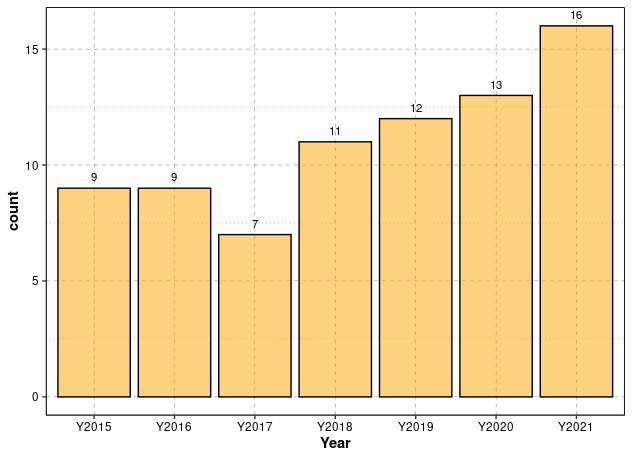
\includegraphics[width=0.6\textwidth]{análisis/numregistersyear.png}
    \caption{Número de grupos por curso académico estudiado.}
    \label{fig:groupsperyear}
\end{figure}

\section{El periodo de tiempo analizado cada año}

En la Tabla \ref{tab:days} se muestra el número de días que dura la práctica cada año. Se puede apreciar que la duración de la práctica que estamos considerando puede variar en función del curso académico.

\begin{table}[H]
\centering
\caption{Número de días que dura la práctica cada año.}
\label{tab:days}
\begin{tabular}{cc}
\hline
\textbf{Year}  & \textbf{Length (days)}  \\ \hline
Y2015 & 32 \\
Y2016 & 23 \\
Y2017 & 29 \\
Y2018 & 17 \\
Y2019 & 27 \\
Y2020 & 16 \\
Y2021 & 38 \\ \hline
\end{tabular}
\end{table}

\section{El conjunto de problemas analizados cada año}

Todos los años hay $9$ problemas de dificultad similar que deben ser resueltos por todos los grupos.

Para aproximarnos al concepto subjetivo de ``dificultad del problema'' vamos a analizar el número de sesiones fallidas que necesita cada alumno para resolverlos por primera vez con respecto al número total de sesiones de ese problema (tasa de fallo) y la duración de este periodo en horas.

\subsection{Dificultad del problema: la tasa de fallo}

La apertura de un problema se corresponde con una sesión de trabajo, la cual puede terminar como fallo (fail) si no se consigue resolver el problema, o éxito (solved) en caso de que se haya resuelto el problema. Así pues, se definirá la tasa de fallo como el cociente entre el número total de sesiones fallidas entre el número total de sesiones de un mismo problema. El boxplot de las tasas de fallo por problema puede verse en la Figura \ref{fig:boxplotfailratio}.

\begin{figure}[H]
    \centering
    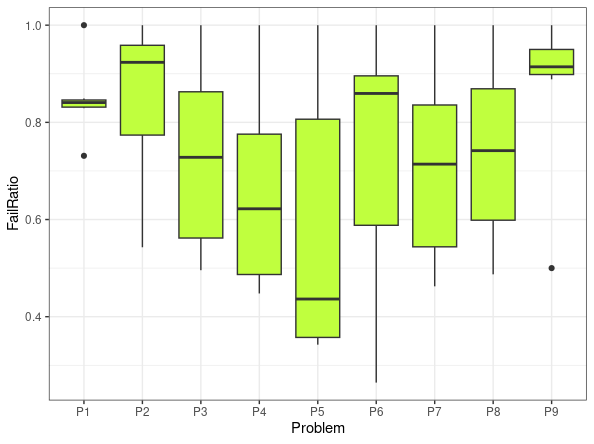
\includegraphics[width=0.6\textwidth]{boxplotfailratioproblem.png}
    \caption{Boxplot de la tasa de fallo (Fail ratio) por problema.}
    \label{fig:boxplotfailratio}
\end{figure}

Tras realizar el test ANOVA de un factor (resultados en la Tabla \ref{tab:ANOVAfailratio}), cuya hipótesis nula establece que la tasa de fallo media de los nueve problemas considerados es la misma, se detecta que las distribuciones de probabilidad de la tasa de fallo son estadísticamente iguales en los distintos problemas ($p = 0.1733 > 0.05$)\footnote{Nótese que hemos establecido un nivel de significancia de $\alpha = 0.05$.}.

% latex table generated in R 4.3.0 by xtable 1.8-4 package
% Sat May 27 20:17:56 2023
\begin{table}[H]
\centering
\caption{Resultados del test ANOVA de un solo factor (tasa de fallo).}
\label{tab:ANOVAfailratio}
\begin{tabular}{lrrrrr}
  \hline
 & Df & Sum Sq & Mean Sq & F value & Pr($>$F) \\ 
  \hline
ndsp[[nVariable]] & 8 & 0.51 & 0.06 & 1.52 & 0.1733 \\ 
  Residuals         & 54 & 2.26 & 0.04 &  &  \\ 
   \hline
\end{tabular}
\end{table}

Además, se ha realizado un test de Tukey por pares de problemas (Tabla \ref{tab:Tukeyfailratio}). En él se observa que casi todos los pares pueden considerarse estadísticamente iguales ($\text{p adj} > 0.2$ en todos ellos) salvo quizá, el par P9-P5 ($\text{p adj} = 0.2$). La Figura \ref{fig:confidenceratiofail} muestra los intervalos de confianza de todas las diferencias entre las distintas parejas de años.

\begin{figure}[H]
    \centering
    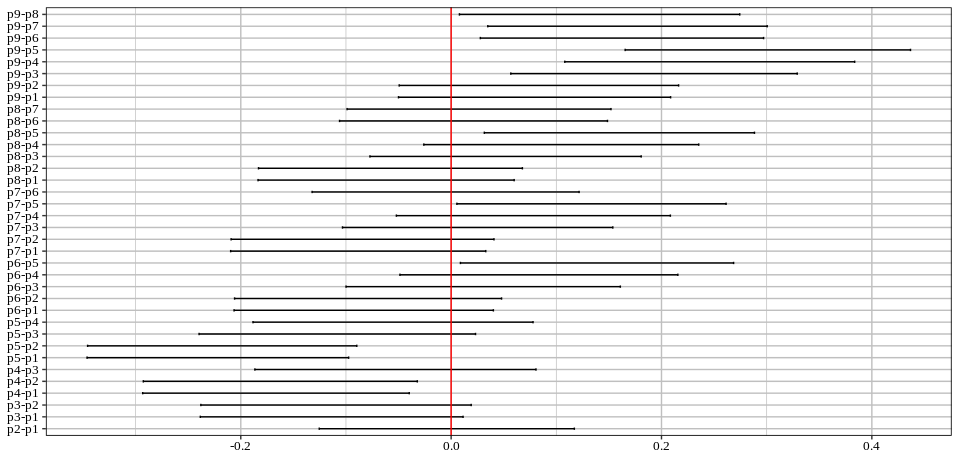
\includegraphics[width=0.80\textwidth]{confidencefailratio.png}
    \caption{Intervalos de confianza de la tasas de fallo de los problemas.}
    \label{fig:confidenceratiofail}
\end{figure}

%Estos datos hay que interpretarlos de manera incremental, pues para resolver un problema Pi requiere las habilidades de Pj(0<=j<i) más habilidades nuevas propias de Pi Periódicamente se incrementa notablemente el nivel de dificultad. P1 es el que más cuesta porque siempre cuesta trabajo empezar, P2-4 son muy parecidos y P5 es un poco más difícil, P6-P8 suben un escalón de dificultad y P9 también.

\subsection{Dificultad del problema: tiempo necesario en resolverlo}

Es el número de horas que transcurren desde que el problema se abre por primera vez hasta que es resuelto por primera vez.

\textbf{Falta imagen.}

De nuevo los tests detectan comportamientos diferentes (ANOVA p=9.27e-5, KW p=8.8e-8).

\textbf{Falta tabla.}

Por pares.

\textbf{Falta tabla.}

Intervalos de confianza.

\textbf{Falta imagen.}

Por lo tanto, se puede ver, dadas las evidencias aportadas que la resolución de cada problema exige respuestas claramente diferentes por parte del alumnado.

\section{Actividad registrada}\label{sec:activityrecorded}

El número de registros y de sesiones de trabajo de cada uno de los años analizados se muestran en la Tabla \ref{tab:records}. Como podemos ver, aunque el curso académico $2021$ registra más actividad que los demás, no es el que presenta un mayor número de sesiones.

\begin{table}[H]
\centering
\caption{Número de registros y sesiones almacenados en el servidor por años.}
\label{tab:records}
\begin{tabular}{ccc}
\hline
\textbf{Year}  & \textbf{Activity Records} & \textbf{Sessions}  \\ \hline
Y2015 & 12088            &  4489  \\
Y2016 & 12525            &  4538  \\
Y2017 & 9088             &  3661  \\
Y2018 & 5705             &  2811  \\
Y2019 & 14475            &  5156  \\
Y2020 & 21188            &  3904  \\
Y2021 & 11961            &  6113  \\ \hline
\end{tabular}
\end{table}

Al ser un servicio 24 horas los 7 días de la semana, los alumnos interactúan con el laboratorio remoto en cualquier día de la semana tal y como puede verse en la Figura \ref{fig:days} y a cualquier hora del día (Figura \ref{fig:hours}).

\begin{figure}[H]
\centering
\subfloat[Histograma de los días de la semana.]{\label{fig:days}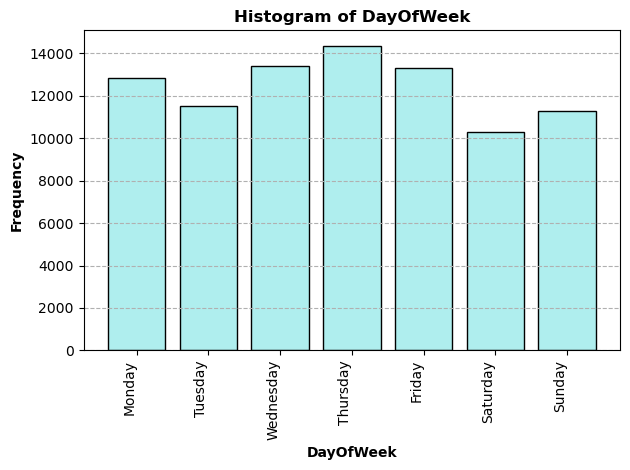
\includegraphics[width=0.47\textwidth]{histogramdayofweek.png}}\qquad
\subfloat[Histograma de las horas del día.]{\label{fig:hours}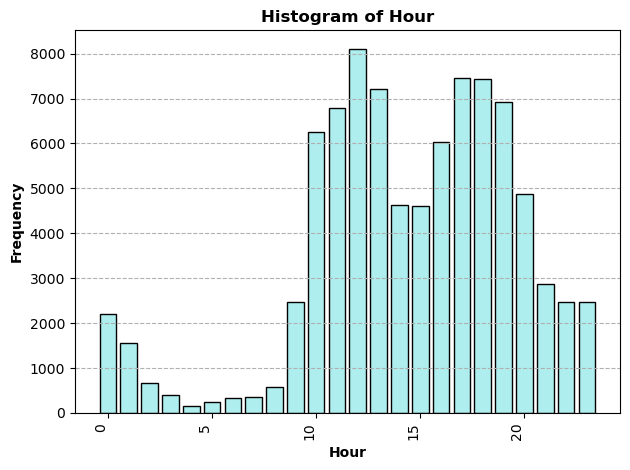
\includegraphics[width=0.47\textwidth]{histogramhour.png}}
\caption{Actividad registrada en el servidor remoto.}
\label{fig:activity}
\end{figure}

El número y tipo de las sesiones de trabajo de cada uno de los grupos puede contemplarse en la Tabla \ref{tab:type}.

\subsection{Análisis de la normalidad de la distribución del número de sesiones}\label{sec:NormalityNumSessions}

En las Figuras \ref{fig:boxplotresiduals} y \ref{fig:histogramresiduals} podemos ver el boxplot de los residuos y el histograma de los mismos.

\begin{figure}[H]
\centering
\subfloat[Boxplot de los residuos del número de sesiones.]{\label{fig:boxplotresiduals}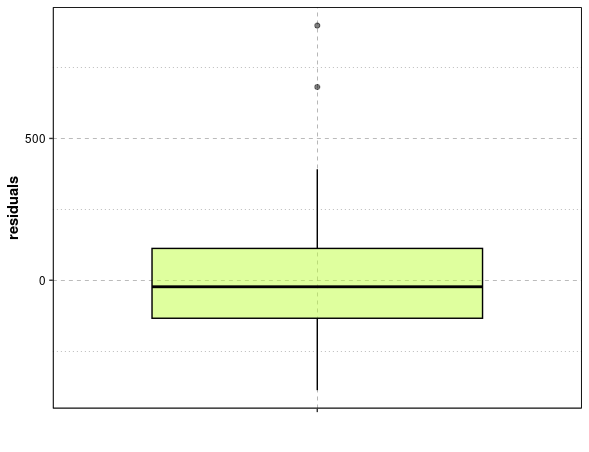
\includegraphics[width=0.47\textwidth]{análisis/residualss.png}}\qquad
\subfloat[Histograma de los residuos del número de sesiones.]{\label{fig:histogramresiduals}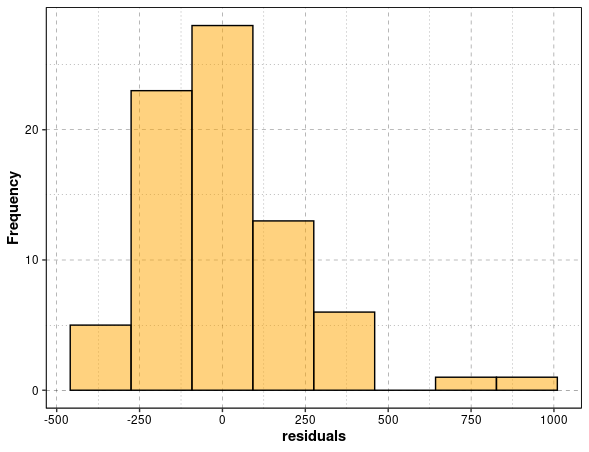
\includegraphics[width=0.47\textwidth]{análisis/histograms.png}}
\caption{Distribución de los residuos del número de sesiones.}
\label{fig:activity}
\end{figure}

A continuación, en las Figuras \ref{fig:densitysessions} y \ref{fig:q-qsessions}, podemos observar que la distribución del número de sesiones no es perfectamente normal pero es casi-normal si eliminaremos algunos outsiders. La línea discontinua vertical marca el valor más probable ($336$ sesiones), lo que muestra un gran esfuerzo por parte del alumnado teniendo en cuenta la duración de la práctica (Tabla \ref{tab:days}).

\begin{figure}[H]
    \centering
    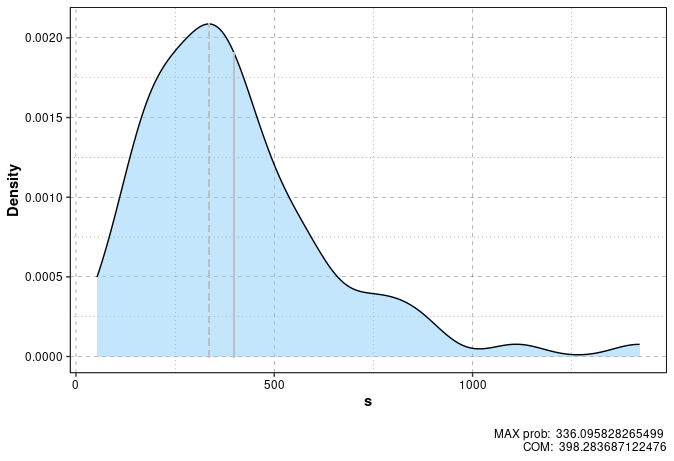
\includegraphics[width=0.70\textwidth]{análisis/densitys.png}
    \caption{Función de densidad de probabilidad del número de sesiones.}
    \label{fig:densitysessions}
\end{figure}


\begin{figure}[H]
    \centering
    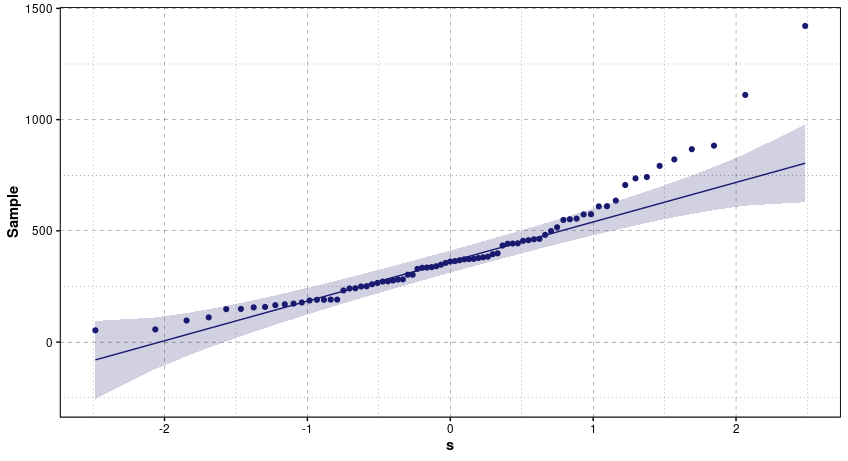
\includegraphics[width=0.75\textwidth]{análisis/qqplots.png}
    \caption{Gráfico Q-Q del número de sesiones.}
    \label{fig:q-qsessions}
\end{figure}

Además, podemos ver en la Figura \ref{fig:outlierss} que hay algunos outliers ($867$, $883$, $1421$ y $1111$) considerando la distribución del número total de sesiones por grupo de alumnos. Segmentando por años, obtenemos los boxplots que se muestran en la Figura \ref{fig:boxplotsessionsyearinitial}. Así pues, eliminaremos aquellos registros que sean outliers en todos los años. Tras realizar la acción anterior, obtenemos la distribución del número de sesiones que se muestra en la Figura \ref{fig:outlierss2}.

\begin{figure}[H]
    \centering
    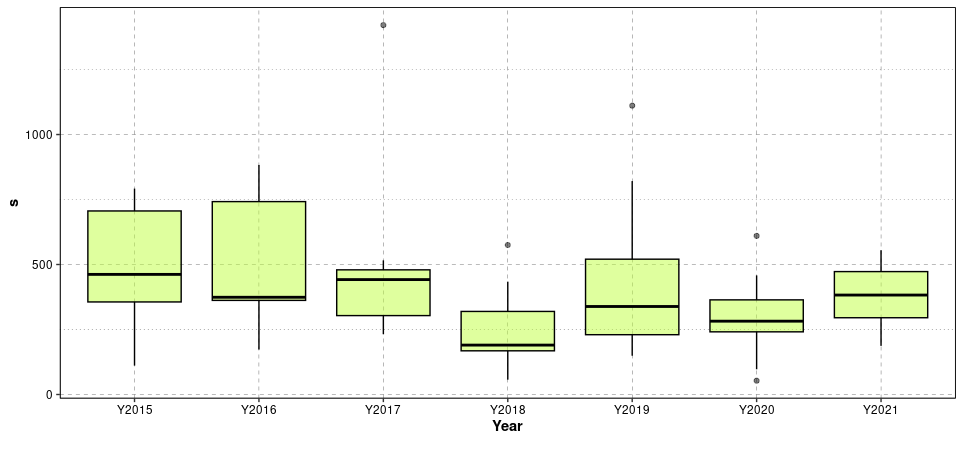
\includegraphics[width=0.60\textwidth]{análisis/boxplotinitials.png}
    \caption{Boxplot del número de sesiones por año inicialmente.}
    \label{fig:boxplotsessionsyearinitial}
\end{figure}

\begin{figure}[H]
    \centering
    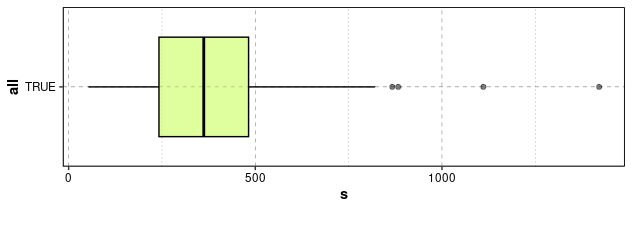
\includegraphics[width=0.60\textwidth]{análisis/outlierss.png}
    \caption{Distribución del número de sesiones inicial.}
    \label{fig:outlierss}
\end{figure}

\begin{figure}[H]
    \centering
    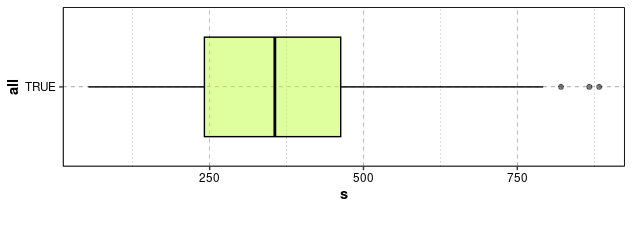
\includegraphics[width=0.60\textwidth]{análisis/outlierss2.png}
    \caption{Distribución del número de sesiones tras la eliminación de algunos outliers.}
    \label{fig:outlierss2}
\end{figure}

Examinamos ahora los bloques significativos entre ellos agrupando los datos en ocho particiones mediante el algoritmo de las K-medias, tal y como se muestra en la Figura \ref{fig:KMeans8}. Los resultados obtenidos pueden verse en las Figuras \ref{fig:KMeans8boxplot} y \ref{fig:KMeans8count}.

\begin{figure}[H]
    \centering
    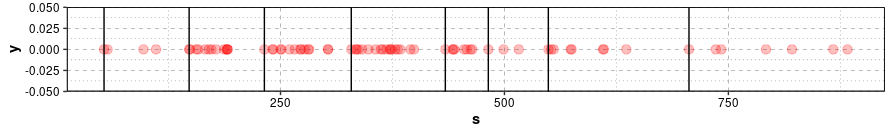
\includegraphics[width=0.6\textwidth]{análisis/KMeanss8.png}
    \caption{Particiones obtenidas con $K = 8$.}
    \label{fig:KMeans8}
\end{figure}

\begin{figure}[H]
\centering
\subfloat[Boxplot de cada una de las particiones.]{\label{fig:KMeans8boxplot}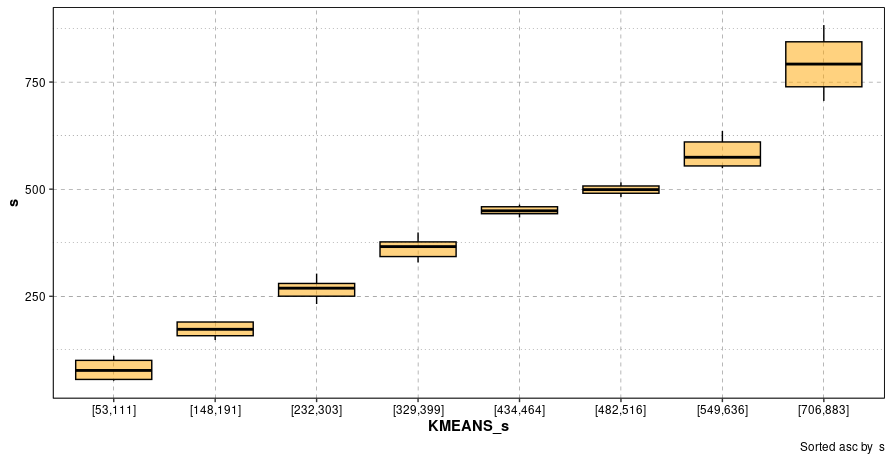
\includegraphics[width=0.47\textwidth]{análisis/KMeanssboxplot.png}}\qquad
\subfloat[Número de grupos por partición.]{\label{fig:KMeans8count}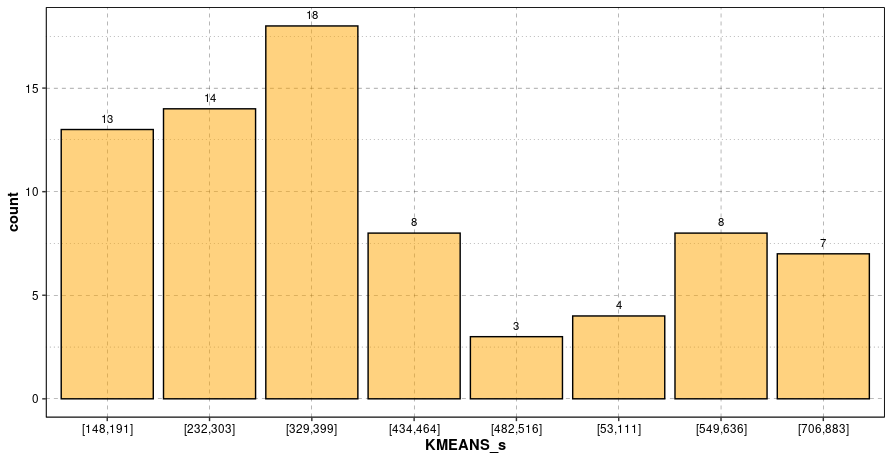
\includegraphics[width=0.47\textwidth]{análisis/KMeansscount.png}}%
\caption{Resultados obtenidos tras aplicar el algoritmo de las $K$-Medias con $K = 8$.}
\label{fig:KMeans8details}
\end{figure}

Nótese que como hemos una obtenido una precisión del $0.9795579\% > 95\%$, no eliminaremos más outliers.

Así pues, tras la eliminación de los outliers correspondientes tanto al número de sesiones como al número de problemas resueltos como veremos en la subsección \ref{sec:NumProblems} (podemos ver la nueva función de densidad en la Figura \ref{fig:normalitys}) se procede a aplicar el test de normalidad de Shapiro-Wilk. Como se obtiene $p-value = 0.003307 < 0.05$, podemos decir que estadísticamente no sigue una distribución normal. No obstante, teniendo en cuenta que el tamaño de la muestra es relativamente pequeño (tenemos un total de $77$ grupos de prácticas), podemos considerar que se trata de una distribución normal.

\begin{figure}[H]
    \centering
    \includegraphics[width=0.70\textwidth]{análisis/normalitys.png}
    \caption{Función de densidad de probabilidad del número de sesiones tras eliminar algunos outliers.}
    \label{fig:normalitys}
\end{figure}

\subsection{Sesiones por cada problema}

En la Figura \ref{fig:boxplotsessionsproblem} podemos ver el boxplot del número de sesiones por problema. Como podemos ver, el problema P1 es mucho más frecuentado que el resto. No obstante, esto se debe la principal diferencia entre el número de sesiones abiertas del problema P1 y restantes se debe a que los alumnos utilizan el primer problema como base de todos los experimentos y para testear las comunicaciones con el servidor. Así pues, el problema P1 es frecuentemente utilizado, no ya sólo al comienzo, sino durante toda la práctica.

\begin{figure}[H]
    \centering
    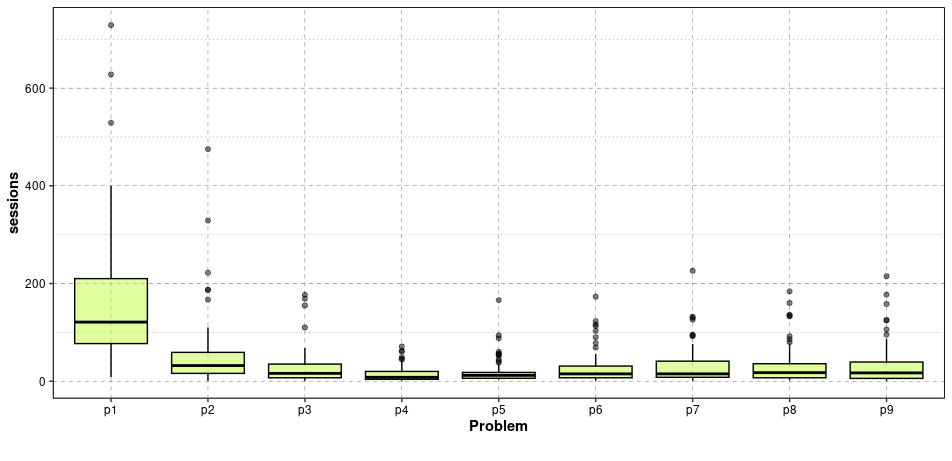
\includegraphics[width=0.6\textwidth]{boxplotsessionsproblem.png}
    \caption{Boxplot del número de sesiones por problema.}
    \label{fig:boxplotsessionsproblem}
\end{figure}

\subsection{Sesiones cada año}\label{sec:ANOVANumSessions}

Como podemos ver en la Figura \ref{fig:boxplotsessionsyear}, las sesiones de trabajo abiertas en el servidor año tras año, parecen seguir la misma distribución de probabilidad.

\begin{figure}[H]
    \centering
    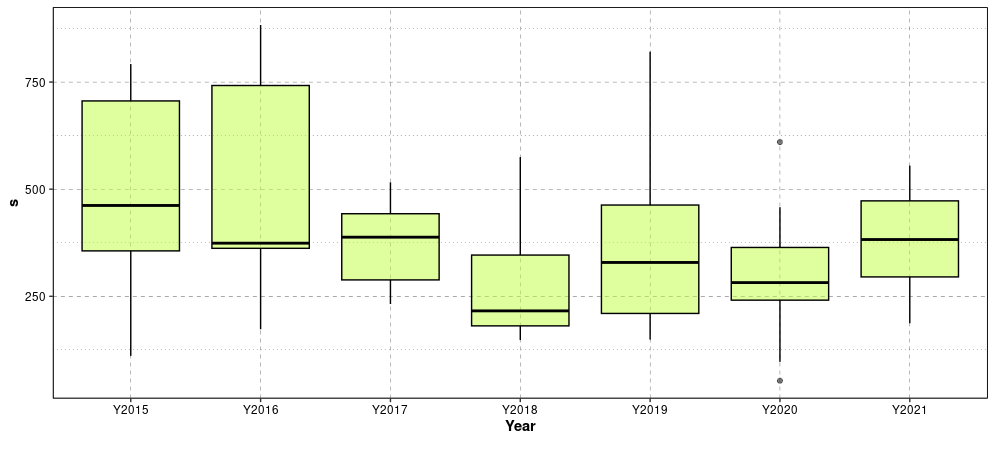
\includegraphics[width=0.60\textwidth]{análisis/boxplotfinals.png}
    \caption{Boxplot del número de sesiones por año tras la eliminación de algunos outliers.}
    \label{fig:boxplotsessionsyear}
\end{figure}

Un resumen de los resultados obtenidos al realizar el test ANOVA se muestra en la Tabla \ref{tab:ANOVAnumsessions}. La hipótesis nula establece que el número de sesiones medio de los siete cursos académicos estudiados es el mismo. Así pues, estableciendo un nivel de significancia de $0.05$, como tenemos que $p = 0.0412 < 0.05$, las diferencias entre las medias podrían ser estadísticamente significativas. Aplicando el test de Kruskal-Wallis, obtenemos un $p-value$ igual a $0.08798 > 0.05$.

% latex table generated in R 4.3.0 by xtable 1.8-4 package
% Sat May 27 18:26:28 2023
\begin{table}[H]
\centering
\caption{Resultados del test ANOVA de un solo factor (número de sesiones).}
\label{tab:ANOVAnumsessions}
\begin{tabular}{lrrrrr}
  \hline
 & Df & Sum Sq & Mean Sq & F value & Pr($>$F) \\ 
  \hline
ndsp[[nVariable]] & 6 & 460434.32 & 76739.05 & 2.34 & 0.0412 \\ 
  Residuals         & 67 & 2197451.96 & 32797.79 &  &  \\ 
   \hline
\end{tabular}
\end{table}

Además, se ha realizado un test de Tukey por pares de años (Tabla \ref{tab:Tukeynumsessions}). En él se observa que todos los pares pueden considerarse estadísticamente iguales ($\text{p adj} > 0.1$ en todos ellos). Así pues, podemos concluir que el número de sesiones abiertas en el servidor sigue la misma distribución de probabilidad año tras año.

La Figura \ref{fig:confidencenumsessions} muestra los intervalos de confianza de todas las diferencias entre las distintas parejas de años. Así pues, consideraremos que el número de sesiones de cada grupo por año es equivalente (las variaciones son debidas al azar). Esto es importante porque indica que el comportamiento más basico de los alumnos, que viene dado por cuantas veces se conectan, es el mismo año tras año.

% latex table generated in R 4.3.0 by xtable 1.8-4 package
% Sat May 27 18:26:44 2023
\begin{table}[ht]
\centering
\caption{Test HSD de Tukey (Honestly-significance-difference) del número de sesiones por años.}
\label{tab:Tukeynumsessions}
\begin{tabular}{rrrrr}
  \hline
 & diff & lwr & upr & p adj \\ 
  \hline
Y2016-Y2015 & 5.44 & -254.06 & 264.95 & 1.00 \\ 
  Y2017-Y2015 & -125.44 & -415.58 & 164.69 & 0.84 \\ 
  Y2018-Y2015 & -223.38 & -476.31 & 29.56 & 0.12 \\ 
  Y2019-Y2015 & -131.05 & -378.48 & 116.38 & 0.68 \\ 
  Y2020-Y2015 & -198.78 & -437.49 & 39.93 & 0.16 \\ 
  Y2021-Y2015 & -116.72 & -346.09 & 112.66 & 0.72 \\ 
  Y2017-Y2016 & -130.89 & -421.03 & 159.25 & 0.81 \\ 
  Y2018-Y2016 & -228.82 & -481.76 & 24.11 & 0.10 \\ 
  Y2019-Y2016 & -136.49 & -383.92 & 110.93 & 0.63 \\ 
  Y2020-Y2016 & -204.22 & -442.93 & 34.49 & 0.14 \\ 
  Y2021-Y2016 & -122.16 & -351.53 & 107.21 & 0.67 \\ 
  Y2018-Y2017 & -97.93 & -382.21 & 186.34 & 0.94 \\ 
  Y2019-Y2017 & -5.61 & -284.99 & 273.78 & 1.00 \\ 
  Y2020-Y2017 & -73.33 & -345.03 & 198.36 & 0.98 \\ 
  Y2021-Y2017 & 8.73 & -254.80 & 272.26 & 1.00 \\ 
  Y2019-Y2018 & 92.33 & -148.20 & 332.86 & 0.90 \\ 
  Y2020-Y2018 & 24.60 & -206.95 & 256.15 & 1.00 \\ 
  Y2021-Y2018 & 106.66 & -115.25 & 328.57 & 0.77 \\ 
  Y2020-Y2019 & -67.73 & -293.25 & 157.80 & 0.97 \\ 
  Y2021-Y2019 & 14.34 & -201.28 & 229.95 & 1.00 \\ 
  Y2021-Y2020 & 82.06 & -123.49 & 287.61 & 0.89 \\ 
   \hline
\end{tabular}
\end{table}

\begin{figure}[H]
    \centering
    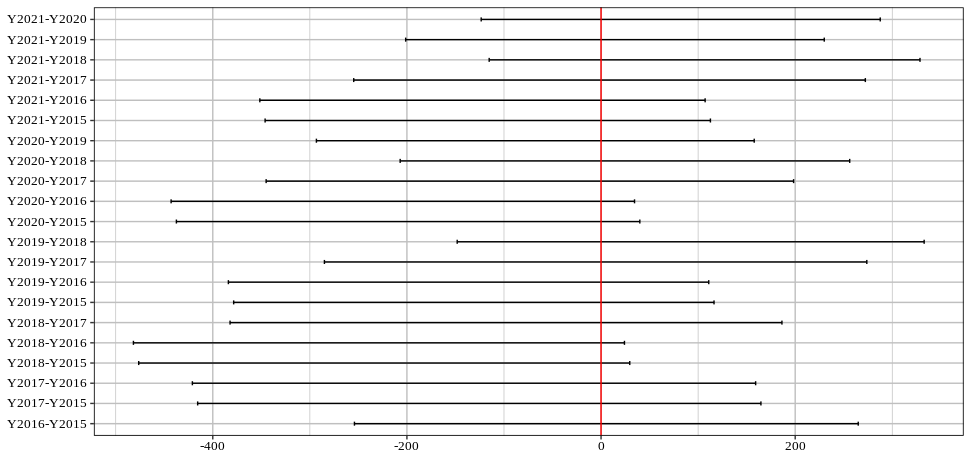
\includegraphics[width=0.80\textwidth]{análisis/confidences.png}
    \caption{Intervalos de confianza del número de sesiones por años.}
    \label{fig:confidencenumsessions}
\end{figure}

\subsection{Análisis de la distribución del número de problemas resueltos}\label{sec:NumProblems}

Además, a partir de los registros almacenados en el servidor se calcularán el número de problemas resueltos por cada grupo de prácticas. Como se puede intuir, se tratará de una variable discreta. En la Figura \ref{fig:initialp} podemos ver que el número de problemas resueltos oscila entre $6$ y $9$.

\begin{figure}[H]
    \centering
    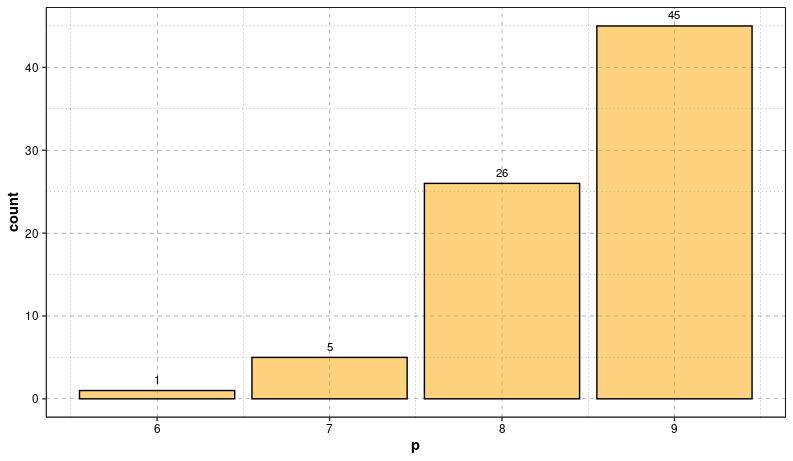
\includegraphics[width=0.6\textwidth]{rendimiento/initialp.png}
    \caption{Distribución del número de problemas resueltos.}
    \label{fig:initialp}
\end{figure}

Además, podemos ver en la Figura \ref{fig:outliersp} que hay un elemento extremo ($6$) considerando la distribución del número de problemas resueltos por grupo de alumnos. Segmentando por años, obtenemos los boxplots que se muestran en la Figura \ref{fig:boxplotproblemsyear}. Así pues, eliminaremos el outlier encontrado puesto que se trata de un valor extremo en todos los años incluidos en este estudio.

\begin{figure}[H]
    \centering
    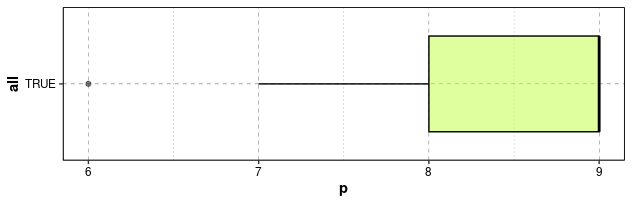
\includegraphics[width=0.60\textwidth]{análisis/outliersp.png}
    \caption{Distribución del número de problemas resueltos inicial.}
    \label{fig:outliersp}
\end{figure}

\begin{figure}[H]
    \centering
    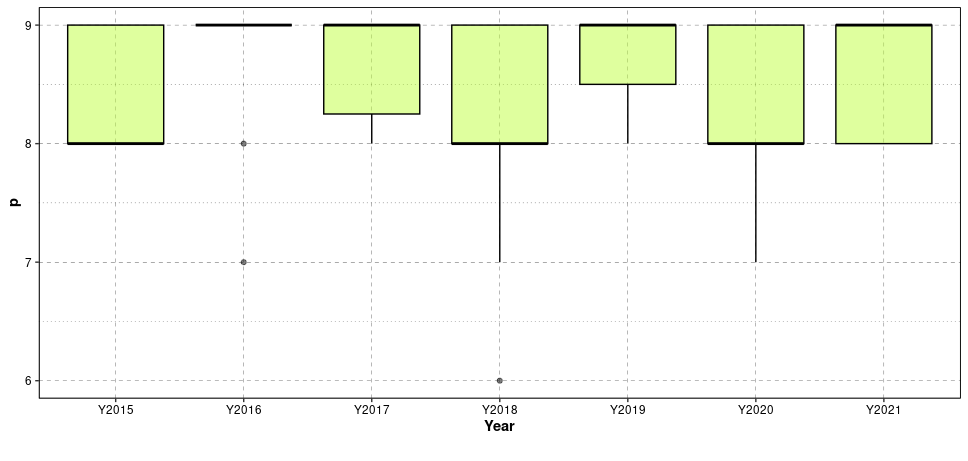
\includegraphics[width=0.60\textwidth]{análisis/boxplotinitialp.png}
    \caption{Boxplot del número de problemas resueltos por año.}
    \label{fig:boxplotproblemsyear}
\end{figure}